\documentclass{standalone}
\usepackage{circuitikz}
\usepackage{amsmath,amssymb}
\usepackage{siunitx}
\begin{document}
	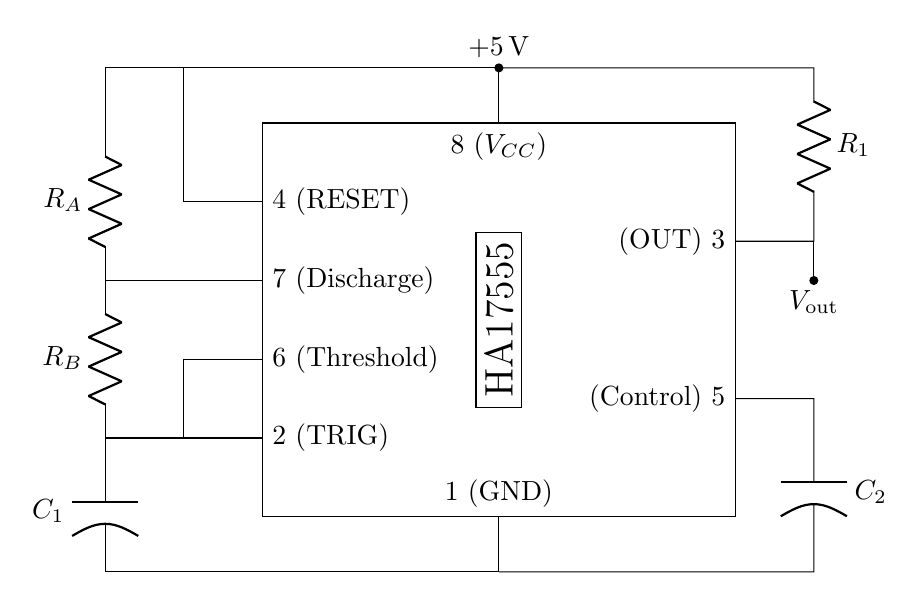
\begin{tikzpicture}
		\draw (0,0) rectangle (6,5);
		\node(1) at (3,0) [above] {1 (GND)};
		\node(2) at (0, 1) [right] {2 (TRIG)};
		\node(6) at (0, 2) [right] {6 (Threshold)};
		\node(7) at (0, 3) [right] {7 (Discharge)};
		\node(4) at (0, 4) [right] {4 (RESET)};
		\node(8) at (3, 5) [below] {8 ($ V_{CC} $)};
		\node(5) at (6,1.5) [left] {(Control) 5};
		\node(3) at (6,3.5) [left] {(OUT) 3};
		\draw (1) |- ++(-5,-1) to[pC, l=$ C_{1} $] ++(0,1.5) |- (2);
		\draw (6) -| (-1, 1);
		\draw (7) -- (-2,3) to[R, a=$ R_{B} $] ++(0,-2);
%		\draw (-2, 3) to[R, l=$ R_{A} $] ++(0,2) -- ++(0,1) -| (8);
		\draw (8) -- ++(0,1) -| (-2,5) to[R, a=$ R_{A} $] ++(0,-2);
		\draw (8) ++(-4,1) |- (4);
		\draw (1) ++ (0,-1) -- ++(4,0) to[pC, a=$ C_{2} $] ++(0,2) |- (5);
		\draw (8) ++(0,1) -- ++(4,0) to[R, l=$ R_{1} $] ++(0,-2) |- (3);
		
		\filldraw (8) ++(0,1) circle [radius=0.05] node[above] {$ +\SI{5}{\volt} $};
		
		\draw (3) -| (7,3) node(out) {};
		\filldraw (out) circle [radius=0.05] node[below] {$ V_{\rm out} $};
		
		\node[draw, rectangle, rotate=90] at (3, 2.5) {\Large HA17555};
	\end{tikzpicture}
\end{document}